\documentclass[12pt]{article}
\usepackage{graphicx}
\usepackage{amsmath}
\usepackage[margin=1in]{geometry}
\begin{document}
\section*{Worksheet A}
\begin{enumerate}
\item Calculate the rate of change from the graph below.

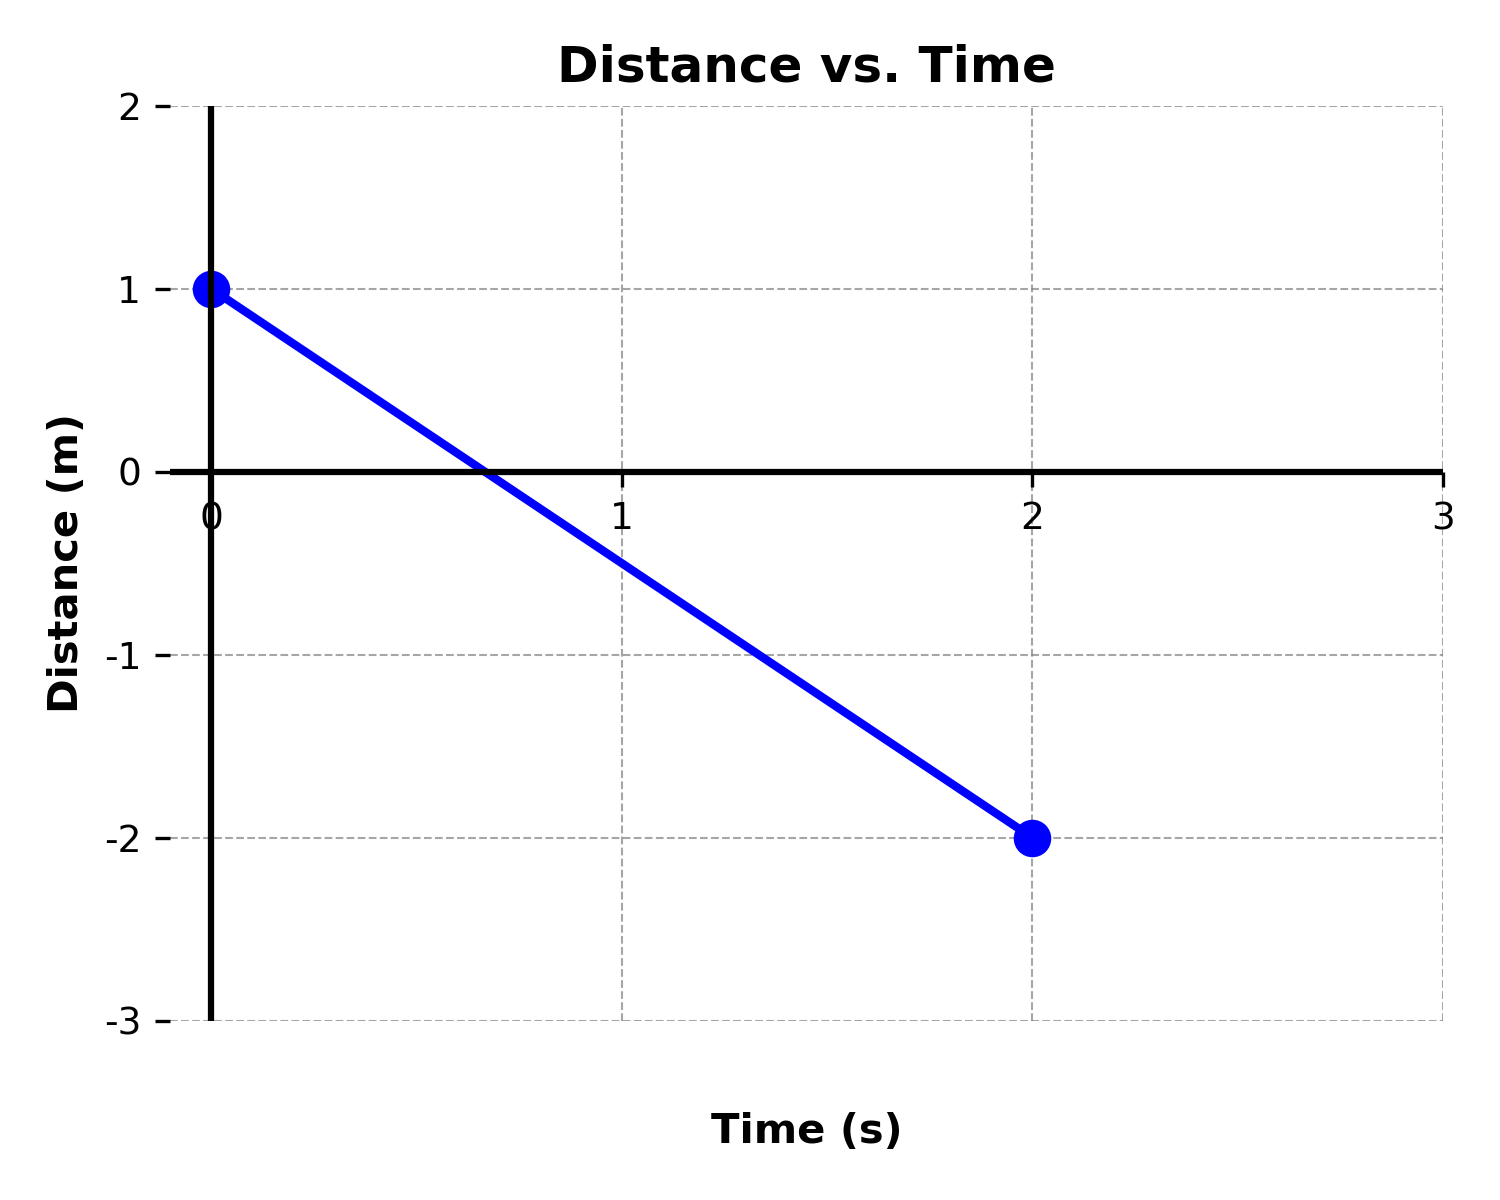
\includegraphics[width=0.6\textwidth]{A_problem_1.png}


\vspace{2cm}  % Add space for students to work
\item Calculate the rate of change from the graph below.

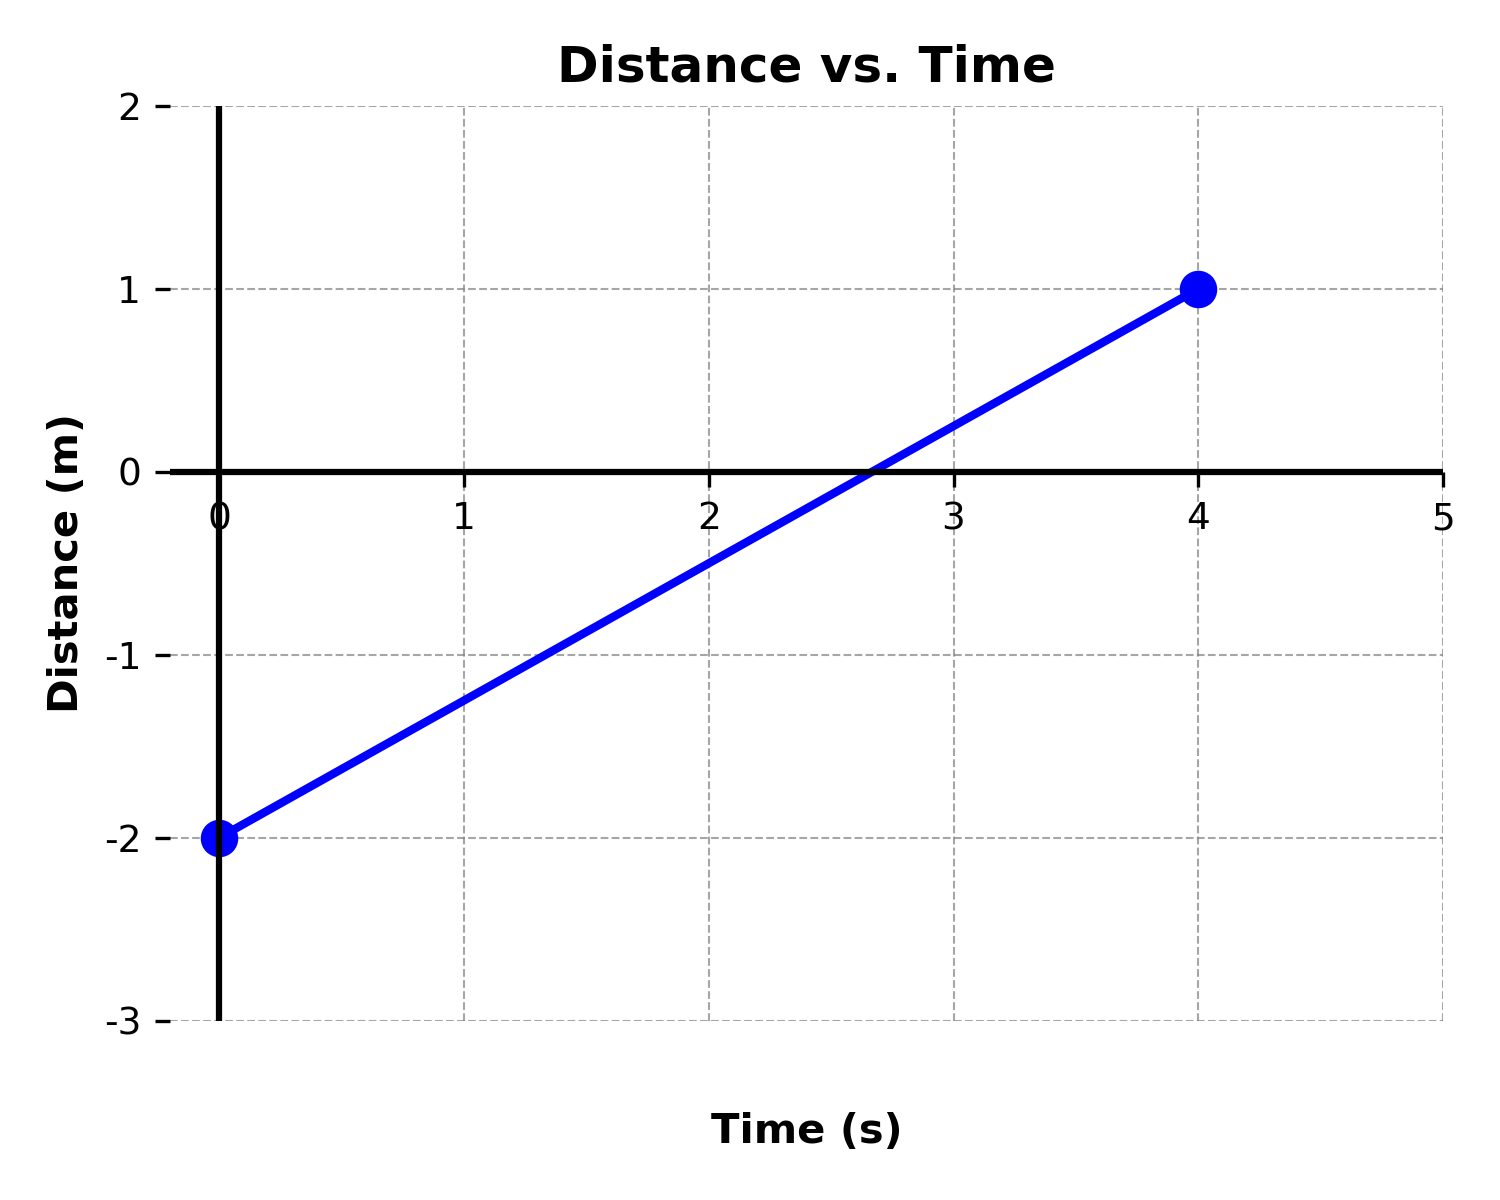
\includegraphics[width=0.6\textwidth]{A_problem_2.png}


\vspace{2cm}  % Add space for students to work
\item Calculate the rate of change from the graph below.

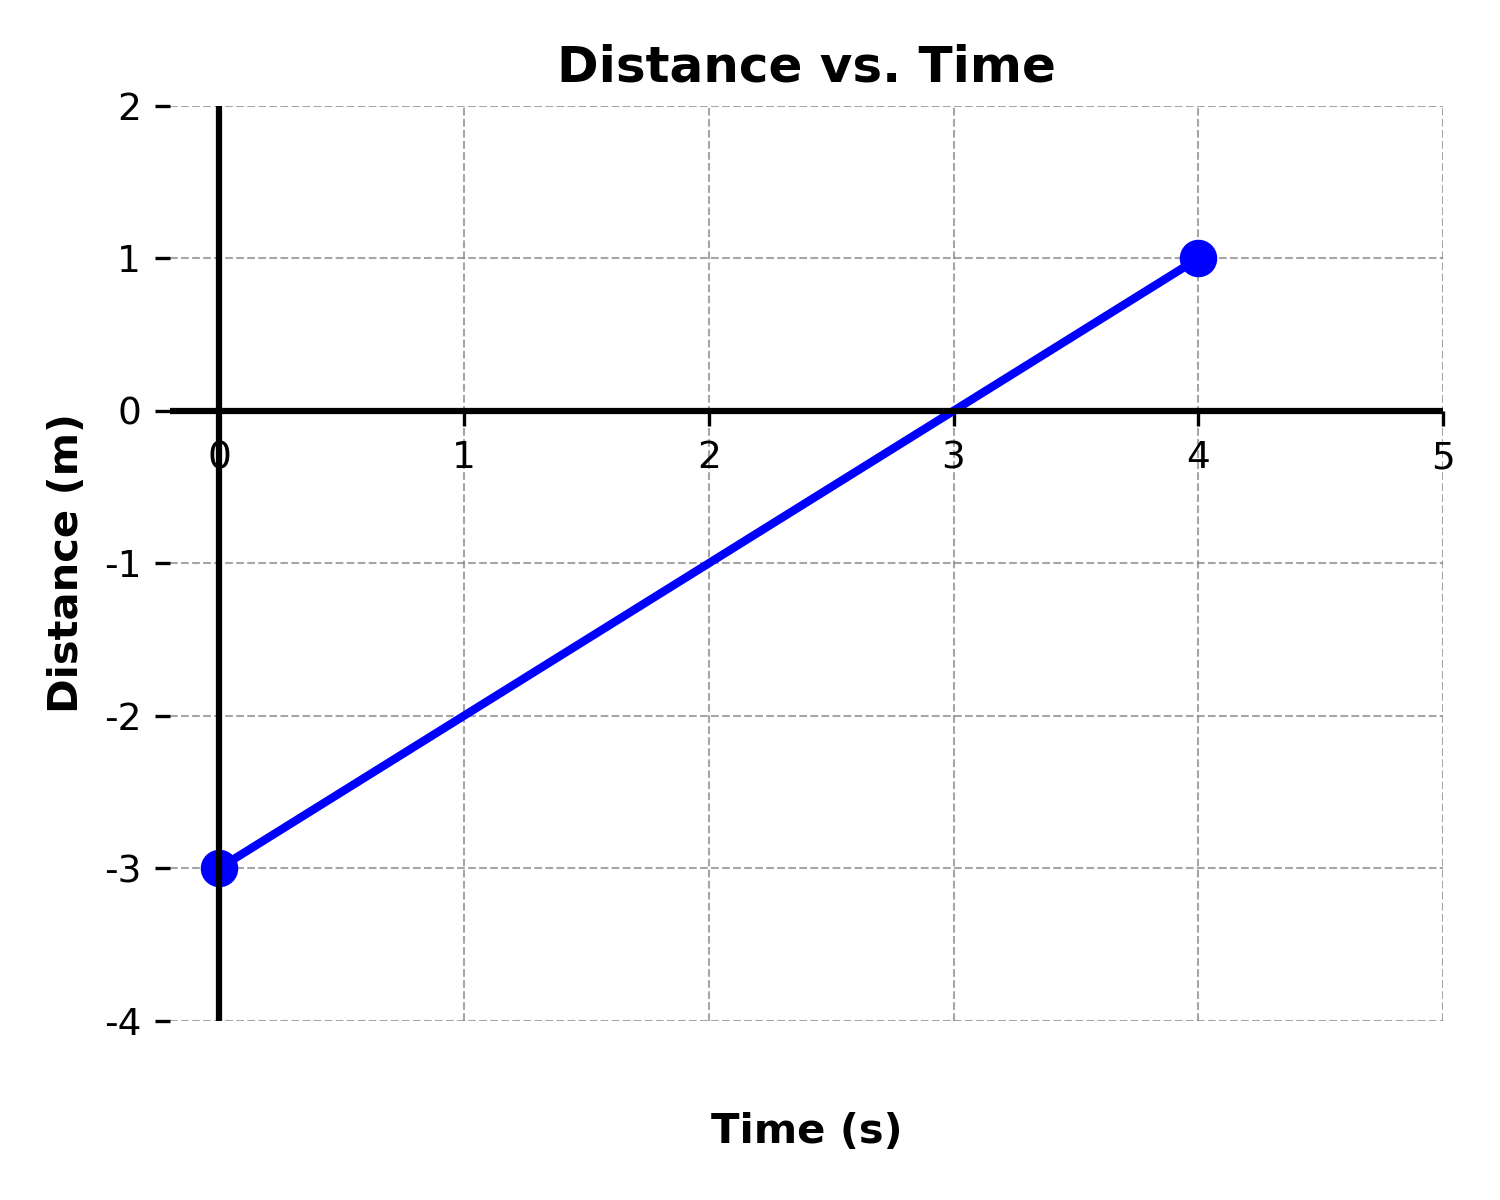
\includegraphics[width=0.6\textwidth]{A_problem_3.png}


\vspace{2cm}  % Add space for students to work
\item Calculate the rate of change from the graph below.

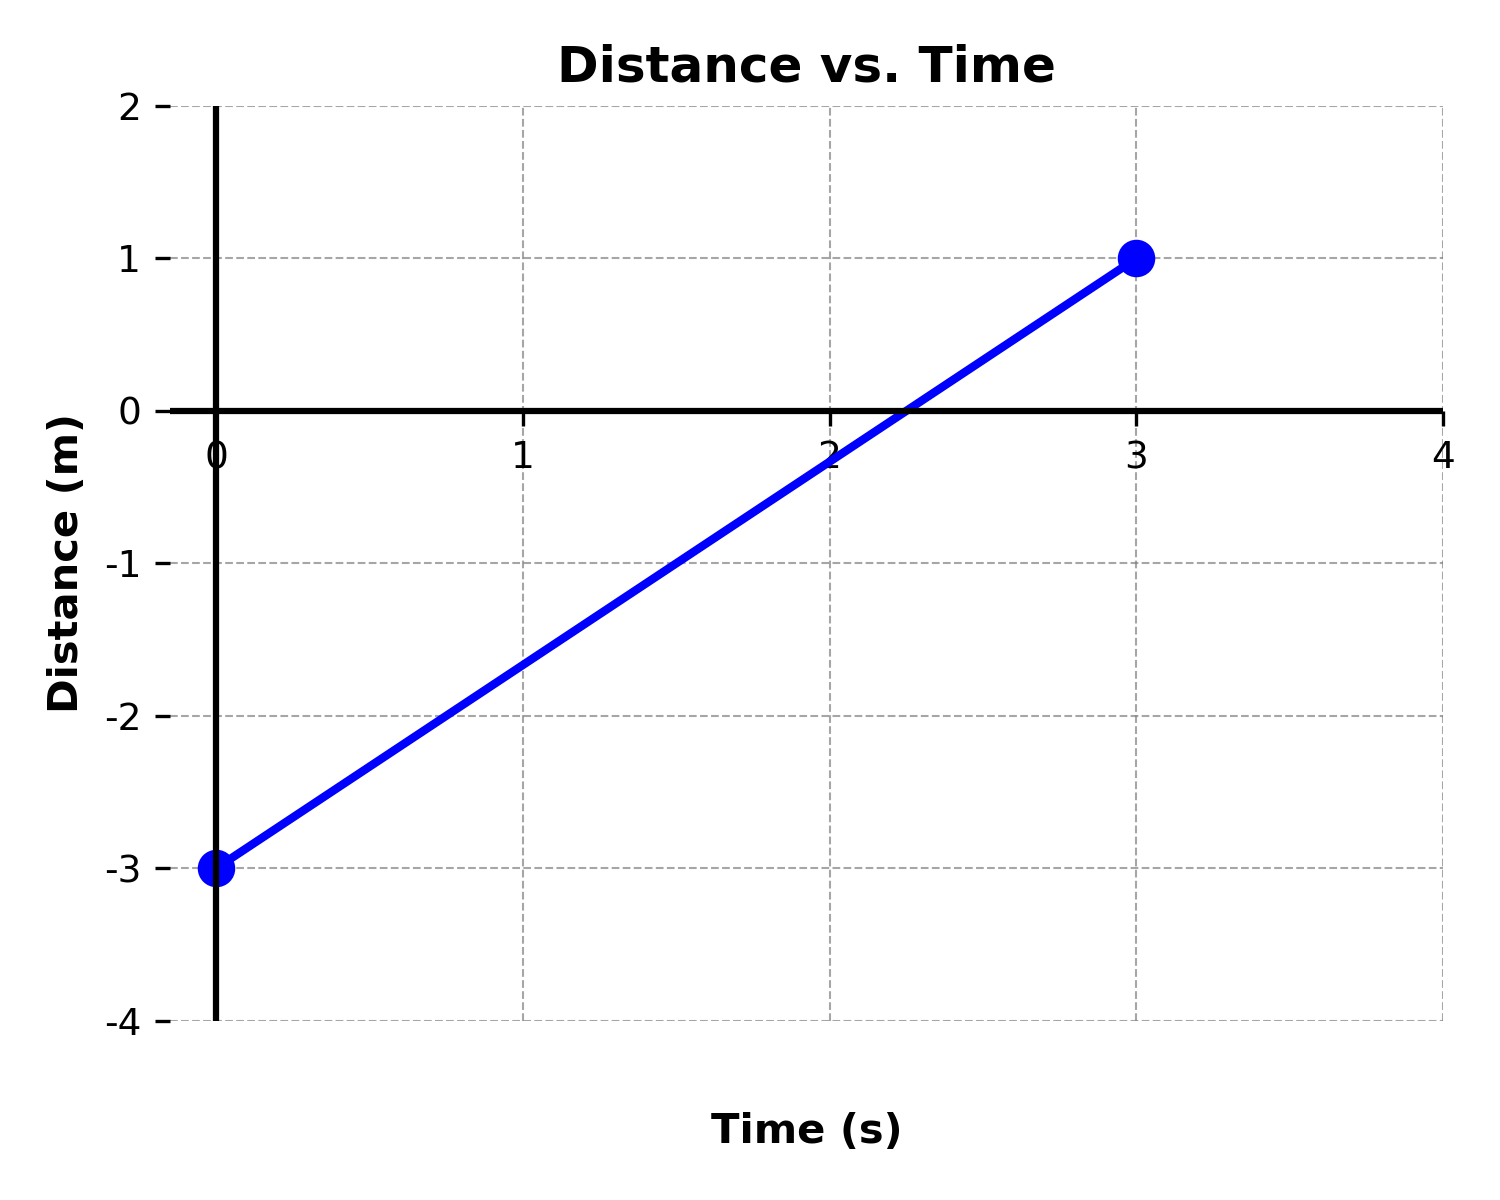
\includegraphics[width=0.6\textwidth]{A_problem_4.png}


\vspace{2cm}  % Add space for students to work
\item Calculate the rate of change from the table below:

\begin{tabular}{|c|c|}
\hline
Time (s) & Distance (m) \\
\hline
0 & -0.5 \\
1 & 1.0 \\
2 & -0.9 \\
4 & 0.3 \\
\hline
\end{tabular}

\vspace{2cm}
\item Calculate the rate of change from the table below:

\begin{tabular}{|c|c|}
\hline
Time (s) & Distance (m) \\
\hline
0 & 1.9 \\
2 & 0.0 \\
3 & 1.7 \\
4 & 1.2 \\
\hline
\end{tabular}

\vspace{2cm}
\item Calculate the rate of change from the table below:

\begin{tabular}{|c|c|}
\hline
Time (s) & Distance (m) \\
\hline
0 & 1.3 \\
1 & -0.9 \\
4 & -1.5 \\
5 & -1.4 \\
\hline
\end{tabular}

\vspace{2cm}
\item Calculate the rate of change from the table below:

\begin{tabular}{|c|c|}
\hline
Time (s) & Distance (m) \\
\hline
0 & 1.7 \\
2 & 0.7 \\
3 & -0.1 \\
5 & -0.5 \\
\hline
\end{tabular}

\vspace{2cm}
\newpage\item An elevator starts at floor -2. After 3 seconds, it is at floor 1. Calculate the rate of change.

\vspace{7cm}
\newpage\item An elevator starts at floor -2. After 4 seconds, it is at floor 1. Calculate the rate of change.

\vspace{7cm}
\end{enumerate}
\newpage
\section*{Answer Key}
\begin{enumerate}
\item The rate of change is $\frac{\Delta y}{\Delta x} = \frac{-2-1}{2-0} = -1.5~\text{units/s}$.

\item The rate of change is $\frac{\Delta y}{\Delta x} = \frac{1--2}{4-0} = 0.75~\text{units/s}$.

\item The rate of change is $\frac{\Delta y}{\Delta x} = \frac{1--3}{4-0} = 1.0~\text{units/s}$.

\item The rate of change is $\frac{\Delta y}{\Delta x} = \frac{1--3}{3-0} = 1.33~\text{units/s}$.

\item The rate of change is $\frac{\Delta y}{\Delta x} = \frac{0.3--0.5}{4-0} = 0.2~\text{units/s}$.

\item The rate of change is $\frac{\Delta y}{\Delta x} = \frac{1.2-1.9}{4-0} = -0.17~\text{units/s}$.

\item The rate of change is $\frac{\Delta y}{\Delta x} = \frac{-1.4-1.3}{5-0} = -0.54~\text{units/s}$.

\item The rate of change is $\frac{\Delta y}{\Delta x} = \frac{-0.5-1.7}{5-0} = -0.44~\text{units/s}$.

\item The rate of change is $\frac{\Delta y}{\Delta x} = \frac{1--2}{3} = 1.0~\text{floors/s}$.

\item The rate of change is $\frac{\Delta y}{\Delta x} = \frac{1--2}{4} = 0.75~\text{floors/s}$.

\end{enumerate}
\end{document}